% Copyright 2005-2016 Airbus-EDF-IMACS-Phimeca
% Permission is granted to copy, distribute and/or modify this document
% under the terms of the GNU Free Documentation License, Version 1.2
% or any later version published by the Free Software Foundation;
% with no Invariant Sections, no Front-Cover Texts, and no Back-Cover
% Texts.  A copy of the license is included in the section entitled "GNU
% Free Documentation License".
\renewcommand{\filename}{docUC_ThresholdExceedance_StrongMaxTest.tex}
\renewcommand{\filetitle}{UC : Validate the design point with the Strong Maximum Test}

% \HeaderNNIILevel
% \HeaderIILevel
\HeaderIIILevel

\index{Threshold Probability!Strong Max Test}




The objective of this Use Case is to explicitate the manipulation of the Strong Max Test. \\

Details on the Strong Max Test  may be found in the Reference Guide (\extref{ReferenceGuide}{see files Reference Guide - Step C -- Strong Maximum Test : a design point validation}{stepC}).\\

The Strong Maximum Test helps to evaluate the quality of the design point resulting from the optimization algorithm. It checks whether the design point computed is :
\begin{itemize}
\item the {\em true} design point, which means a global maximum point,
\item a {\em strong} design point, which means that there is no other local maximum located on the event boundary and which likelihood is slightly inferior to the design point one.
\end{itemize}
This verification is very important in order to give sense to the FORM and SORM approximations .\\


We briefly recall here the main principles of the test, drawn on figure (\ref{SMT}).\\
The objective is to detect all the points $\tilde{P}^*$ in the ball of radius $R_{\varepsilon} = \beta(1+\delta_{\varepsilon})$ which are potentially the real design point (case of $\tilde{P}_2^*$) or which contribution to $P_f$ is not negligeable as regards the approximations Form and Sorm (case of $\tilde{P}_1^*$). The contribution of a point is considered as negligeable when its likelihood in the $\bdU$-space is more than $\varepsilon$-times lesser than the design point one. The radius $R_{\varepsilon}$ is the distance to the $\bdU$-space center upon which points are considered as negligeable in the evaluation of $P_f$.\\

In order to catch the potential points located on the sphere of radius $R_{\varepsilon}$ (frontier of the zone of prospection), it is necessary to go a little further more : that's why the test samples the sphere of radius  $R = \beta(1+\tau \delta_{\varepsilon})$, with $\tau >0$.\\

Points on the sampled sphere which are in the vicinity of the design point $P^*$ are less interesting than those verifying the event and located {\itshape far} from the design point : these last ones might reveal a potential $\tilde{P}^*$ which contribution to $P_f$ has to be taken into account. The  vicinity of the design point is defined with the angular parameter $\alpha$ as the cone centered on $P^*$ and of half-angle $\alpha$.\\

The number $N$ of the simulations sampling the sphere of radius $R$ is determined  to ensure that the test detect with a probability greater than $(1 - q)$ any point verifying the event and outside the design point vicinity. \\

\begin{figure}[H]
  \begin{center}
    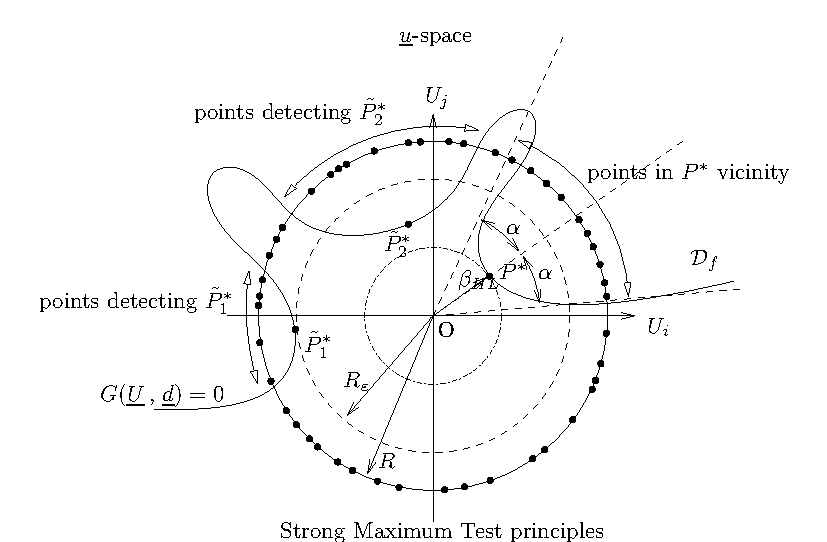
\includegraphics[scale=0.85]{Figures/FigureStrongMaxTest.pdf}
    \caption{The Strong Maximum Test to validate the quality of the design point : unicity and strongness}
    \label{SMT}
  \end{center}
\end{figure}

The vicinity of the Design Point  is the arc of the sampled sphere which is inside the half space which frontier is the linearized limit state function at the Design Point (see figure (\ref{vicinity}) : the vicinity is the arc included in the half space $D_1$).\\

\begin{figure}[H]
  \begin{center}
    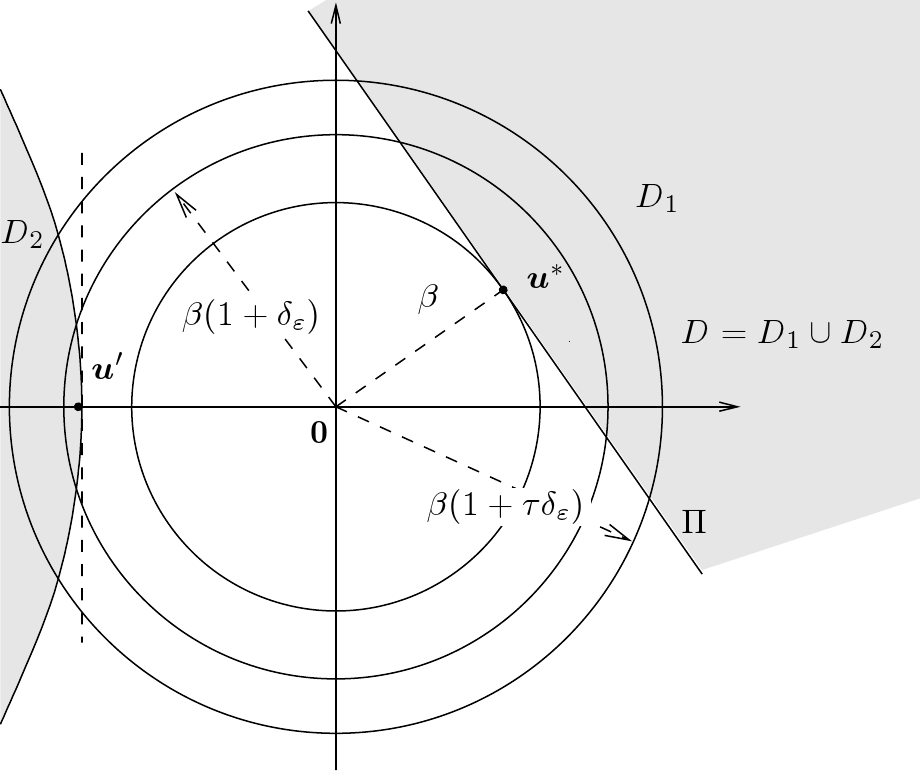
\includegraphics[width = 8cm]{Figures/StrongMaxTest_vicinity.png}
    \caption{Vicinity of the Design Point in the standard space : the half space $D_1$}
    \label{vicinity}
  \end{center}
\end{figure}

The Strong Maximum Test proceeds as follows. The User selects the parameters :
\begin{itemize}
\item the importance level $\varepsilon$,
\item the accuracy level $\tau$,
\item the confidence level $(1 - q)$ or the number of points $N$ used to sample the sphere. The parameters are deductible from one other.
\end{itemize}
The Strong Maximum Test will sample the sphere of radius  $\beta(1+\tau  \delta_{\varepsilon})$, where  $\delta_{\varepsilon} =        \sqrt{1 - 2 \frac{\ln(\varepsilon)}{\beta^2}}- 1$. \\
The test will detect with a probability greater than $(1 - q)$ any point of $\cD_f$ which contribution to $P_f$ is not negligeable (i.e. which density value in the $\bdU$-space is greater than $\varepsilon$ times the density value  at the design point).\\

The Strong Maximum Test provides :
\begin{itemize}
\item set 1 : all the points detected on the sampled sphere  that are in $\cD_f$ and outside the design point vicinity, with the corresponding value of the limit state function. These points are given thanks to the method {\em getFarDesignPointVerifyingEventPoints}. The respective values of the limit state function at these points are given thanks to the method {\em getFarDesignPointVerifyingEventValues}.
\item set 2 : all the points detected on the sampled sphere  that are in $\cD_f$ and in the design point vicinity, with the corresponding value of the limit state function. These points are given thanks to the method {\em getNearDesignPointVerifyingEventPoints}. The respective values of the limit state function at these points are given thanks to the method {\em getNearDesignPointVerifyingEventValues}.
\item set 3 : all the points detected on the sampled sphere  that are outside $\cD_f$ and  outside the design point vicinity, with the corresponding value of the limit state function. These points are given thanks to the method {\em getFarDesignPointViolatingEventPoints}. The respective values of the limit state function at these points are given thanks to the method {\em getFarDesignPointViolatingEventValues}.
\item set 4 : all the points detected on the sampled sphere  that are outside $\cD_f$ but in the vicinity of the design point, with the corresponding value of the limit state function. These points are given thanks to the method {\em getNearDesignPointViolatingEventPoints}. The respective values of the limit state function at these points are given thanks to the method {\em getNearDesignPointViolatingEventValues}.
\end{itemize}
Points are described by their coordinates  in the $\bdX$-space.\\

The Reference Guide helps to quantify the parameters of the test.\\

As the Strong Maximum Test involves the computation of $N$ values of the limit state function, which is computationally intensive, it is interesting to have more than just an indication about the quality of $\vect{OP}^*$. In fact, the test gives some information about the trace of the limit state function on the sphere of radius $\beta(1+\tau \delta_{\varepsilon})$ centered on the origin of the $\bdU$-space. Two cases can be distinguished:
\begin{itemize}
\item Case 1: set 1 is empty. We are confident on the fact that $\vect{OP}^*$ is a design point verifying the hypothesis according to which most of the contribution of $P_f$ is concentrated in the vicinity of $\vect{OP}^*$. By using the value of the limit state function on the sample $(\vect{U}_1, \dots, \vect{U}_N)$, we can check if the limit state function is reasonably linear in the vicinity of $\vect{OP}^*$, which can validate the second hypothesis of FORM. \\
  If the behaviour of the limit state function is not linear, we can decide to use an importance sampling version of the Monte Carlo method for computing the probability of failure (refer to \extref{ReferenceGuide}{Reference Guide - Step C -- Importance sampling}{stepC}). However, the information obtained through the Strong Max Test, according to which $\vect{OP}^*$ is the actual design point, is quite essential : it allows to construct an effective importance sampling density, e.g. a multidimensional gaussian distribution centered on $\vect{OP}^*$.
\item Case 2:   set 1 is not empty. There are two possibilities:
  \begin{enumerate}
  \item We have found some points that suggest that $\vect{OP}^*$ is not a strong maximum, because for some points of the sampled sphere, the value taken by the limit state function is slightly negative;
  \item We have found some points that suggest that $\vect{OP}^*$ is not even the global maximum, because for some points of the sampled sphere, the value taken by the limit state function is very negative.\\
    In the first case, we can decide to use an importance sampling version of the Monte Carlo method for computing the probability of failure, but with a mixture of e.g. multidimensional gaussian distributions centered on the $U_i$ in $\cD_f$ (refer to \extref{ReferenceGuide}{Reference Guide - Step C -- Importance Sampling}{stepC}).
    In the second case, we can restart the search of the design point by starting at the detected $U_i$.
  \end{enumerate}
\end{itemize}

\requirements{
  \begin{description}
  \item[$\bullet$] the event of the FORM analysis described in the standard space {\itshape myStandardEvent}
  \item[type:] StandardEvent
  \item[$\bullet$] the design point expressed in the standard space {\itshape standardSpaceDesignPoint}
  \item[type:] a NumericalPoint
  \end{description}
}
             {
               \begin{description}
               \item[$\bullet$] all the points in $\cD_f$ and outside the design point vicinity : {\em potentialDesignPoints}
               \item[type:] a NumericalSample
               \item[$\bullet$] all the points in $\cD_f$ and inside the design point vicinity : {\em vicinityDesignPoint}
               \item[type:] a NumericalSample
               \item[$\bullet$] all the points outside $\cD_f$ and outside the design point vicinity : {\em farSecurityPoints}
               \item[type:] a NumericalSample
               \item[$\bullet$] all the points outside $\cD_f$ and inside the design point vicinity : {\em vicinitySecurityPoints}
               \item[type:] a NumericalSample
               \end{description}
             }

             \textspace\\

             Python script for this UseCase :

             \inputscript{script_docUC_ThresholdExceedance_StrongMaxTest}
